\chapter{Техническая реализация}
\label{sec:chap3}

\section{Описание реализации}

\begin{figure}[!h]
\centering
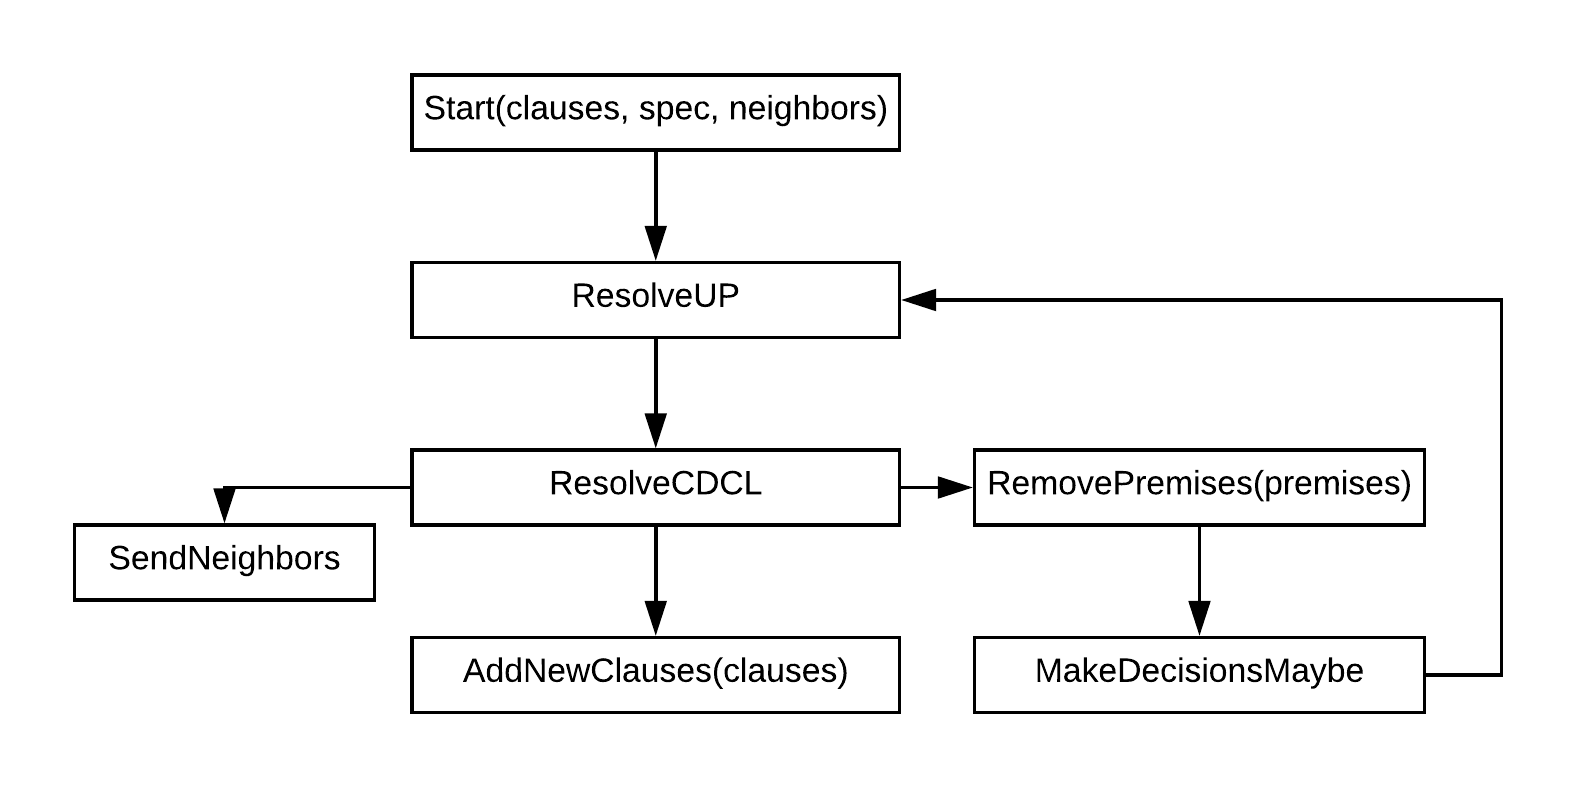
\includegraphics[scale=0.9]{actorProcess.png}
\caption{Сообщения внутри одного актора.}\label{fig:actorProcess}
\end{figure}

На рисунке \ref{fig:actorProcess} описано то, как ведёт себя один актор, для случая статической специализации.
Изначально мы посылаем каждому актору все сообщения с помощью тега \emph{Start}.
\begin{lstlisting}[language=scala]
    case Start(initialClauses, actors) =>
      onReceiveStart(initialClauses, actors)
      self ! ResolveUnitPropagation
\end{lstlisting}

Далее выполняется поиск резолюций -- для этого перебирается клоз, выбирается один литерал, для остальных же ищем соответствующую пару в структуре данных, поддерживающей поиск унифицирующих литералов. Далее применяем унификатор к выбранному литералу, и добавляем его в базу данных внутри этого актора.

После стадии поиска резолюций, начинается выявление конфликтов. Для поиска конфликтов мы должны перебрать пару литералов, где хотя бы один был выведен на последней итерации, и попытаться подобрать унификатор. Если это получилось, то мы нашли локальный конфликт. В локальном конфликте мы должны проверить существование предположений. Если они есть, то применить правило \emph{CDCL}. Если же их нет, то мы должны взять остаточный клоз и разослать его всем соседям в нашей топологии. Если остаточный клоз тоже пустой, то мы нашли конфликт и необходимо завершить работу всех акторов.

Если на последней итерации стадий \emph{CDCL} и \emph{Unit-Propagation Resolution} не было выявлено новых литералов, то нам нужно сделать предположение. Выбор предположений -- отдельная очень обширная для изучения тема, в которой можно использовать методы обучения с подкреплением, различные простые эвристики [\texttt{TODO: найти ссылку, точно была}]. Однако в рамках этой реализации предположение выбирается случайным образом.

\section{Доказательство полноты}
\texttt{TODO: промоделировать это в нашем исчислении}
\section{Оценка сложности для задачи \emph{Принцип Дирихле}}
В резолюционном исчислении сложно оценивать сложность общего алгоритма, поэтому чаще всего оценивается на конкретных задачах. Одной из таких классических задач является \emph{Принцип Дирихле}. 
\texttt{TODO: написать здесь доказательство оценки}
\section{Оценка производительности}
\texttt{TODO: выложить здесь графики с запусков на \emph{TPTP}}

